\documentclass[conference]{IEEEtran}
\usepackage{times}

% numbers option provides compact numerical references in the text. 
\usepackage[numbers]{natbib}
\usepackage{multicol}
\usepackage[bookmarks=true]{hyperref}
\usepackage{graphicx}
\usepackage{amsmath,amsfonts,amssymb}

\graphicspath{ {./graphics/} }

\pdfinfo{
   /Author (Mingyo Seo)
   /Title  (Robots: Our new overlords)
   /CreationDate (D:20101201120000)
   /Subject (Robots)
   /Keywords (Robots;Overlords)
}

\begin{document}

% paper title
\title{CS391L HW1: Eigen Digits}

% You will get a Paper-ID when submitting a pdf file to the conference system
\author{Mingyo Seo}

\author{\authorblockN{Mingyo Seo}
\authorblockA{
% Department of Electrical and\\Computer Engineering\\
%Georgia Institute of Technology\\
%Atlanta, Georgia 30332--0250\\
UT EID: ms84662\\
Email: mingyo@utexas.edu}}
%\and
%\authorblockN{Homer Simpson}
%\authorblockA{Twentieth Century Fox\\
%Springfield, USA\\
%Email: homer@thesimpsons.com}
%\and
%\authorblockN{James Kirk\\ and Montgomery Scott}
%\authorblockA{Starfleet Academy\\
%San Francisco, California 96678-2391\\
%Telephone: (800) 555--1212\\
%Fax: (888) 555--1212}}


% avoiding spaces at the end of the author lines is not a problem with
% conference papers because we don't use \thanks or \IEEEmembership


% for over three affiliations, or if they all won't fit within the width
% of the page, use this alternative format:
% 
%\author{\authorblockN{Michael Shell\authorrefmark{1},
%Homer Simpson\authorrefmark{2},
%James Kirk\authorrefmark{3}, 
%Montgomery Scott\authorrefmark{3} and
%Eldon Tyrell\authorrefmark{4}}
%\authorblockA{\authorrefmark{1}School of Electrical and Computer Engineering\\
%Georgia Institute of Technology,
%Atlanta, Georgia 30332--0250\\ Email: mshell@ece.gatech.edu}
%\authorblockA{\authorrefmark{2}Twentieth Century Fox, Springfield, USA\\
%Email: homer@thesimpsons.com}
%\authorblockA{\authorrefmark{3}Starfleet Academy, San Francisco, California 96678-2391\\
%Telephone: (800) 555--1212, Fax: (888) 555--1212}
%\authorblockA{\authorrefmark{4}Tyrell Inc., 123 Replicant Street, Los Angeles, California 90210--4321}}


\maketitle

\IEEEpeerreviewmaketitle

\begin{abstract}
This assignment aims at optical character recognition (OCR) for hand-written digit characters. In specific, we extract features from raw pixel images by using the principal component analysis (PCA) method. The features mapped from the pixel space to the PCA eigenspace will be used for classification by comparing the features of k-nearest neighbor (KNN) in training samples. We evaluated this method by the MNIST handwritten digit sets and discussed how parameters affect the OCR model's accuracy and computation requirements.
\end{abstract}

\section{Introduction} % Introduce your problem and the overall plan for approaching your problem

The problem of classifying digits is well studied in previous works, and 
there have been many methods explored to solve this problem, such logistic regressions \cite{bishop1995neural}, support vector machines \cite{decoste2002training}, CNNs\cite{lecun1998gradient}, etc.
In this paper, we implemented an OCR classification model that performs PCA to extract features from raw images and classifies them by KNN methods. We also studied the effects of parameters on the model's accuracy and computation requirements. The answers to the HW1 questions are included in the following sections.\begin{itemize}
\item Fig. \ref{fig:eig_vecs}: Visualization of eigenvectors
\item Fig. \ref{fig:pca_5}-\ref{fig:pca_784}: Visualization of reconstructed test digits
\item Fig. \ref{fig:pca_test}: Correlation between accuracy and eigenvectors
\item Fig. \ref{fig:sample_test}: Correlation between accuracy and training set
\end{itemize}

\section{Method}
\label{sec:method}
\subsection{MNIST dataset} % Introduce your problem and the overall plan for approaching your problem
The MNIST dataset consists of a training set of 60,000 samples and a test set of 10,000 samples.
Samples are given by images of handwriting digit characters along with 10 different labels (0-9).
An image has $28 \times 28$ gray-scale pixels, and each pixel has an integer value in the range from 0 to 255 (8bits).
In this assignment, our classifier model uses a flattened 784-length vector of pixel images as an input.
A label is given as a 10-length vector: only one element is 1 to indicate the class of the character and the others are 0.
\subsection{Principal Component Analyais} % Introduce your problem and the overall plan for approaching your problem
\label{subsec:pca}
PCA allows to extract important pattern features in the forms of eigenvectors.
Let $X = [\boldsymbol{x}_1; \boldsymbol{x}_2; ... ; \boldsymbol{x}_N]$ to be the images in the training set of $N$ samples, and 
$\bf{x}_i$ be the $i$th flatten 784-length image vector.
Then, the covariance matrix $A$ of the training set $X$ is given as,
\begin{equation}
A = {1\over{N}}\sum_{i=1}^{N} (\boldsymbol{x}_i - \boldsymbol\mu)^\intercal (\boldsymbol{x}_i-\boldsymbol\mu),
\end{equation}
where $\boldsymbol\mu$ is a 784-length mean pixel vector of the $N$ samples as,
\begin{equation}
\boldsymbol\mu = {1\over{N}}\sum_{i=1}^{N} \boldsymbol{x}_i.
\end{equation}
The subtraction of $\boldsymbol\mu$ shifts the means of the pixel samples to be zero, which allows extracting pattern features from eigenvectors of the covariance matrix $A$.
Let $U = [\boldsymbol{u}_1; \boldsymbol{u}_2; ... ; \boldsymbol{u}_{284}]$ to an unitary matrix of $A$, and $\boldsymbol{u}_k$ be an unit eigen vector, where the index $k$ is sorted in dscending order of the corresponding eigen values $\lambda_k$. Here, an eigen vector $\boldsymbol{u}_k$ is orthogonal to each other and represents pattern features in the eigen space. 
Eigenvalues are correlated weightage of the corresponding eigenvectors in training pixel images. 
Therefore, we can select the eigenvectors of the $M$ largest eigenvalues to extract important features. 
The mapping from the pixel space to the selective eigenspace of either training or test image sample $\boldsymbol{x}_j$ is given as,
\begin{equation}
\boldsymbol{x}_j U_M = \boldsymbol\alpha_j U_M = \sum_{k=1}^{M} \alpha_{j,k} \boldsymbol{u}_k 
\end{equation}
where $U_M = [\boldsymbol{u}_1; \boldsymbol{u}_2; ... ; \boldsymbol{u}_{M}]$.
Here, $\boldsymbol\alpha = [\alpha_{j,1}, \alpha_{j,2}, ..., \alpha_{j,M}]$ represents pattern features of an sample image $\boldsymbol{x}_j$. 
This operation removes minor features of $\boldsymbol{u}_{M+1}, ..., \boldsymbol{u}_{284}$ from the original image data. 
By comparing $\boldsymbol\alpha_j$ of an image $\boldsymbol{x}_j$ with the ones of training samples, we can classify the digits.
Since the above opreation reduce the components in the eigen space, reconstruction of reduced components can be processed by mapping $\boldsymbol\alpha$ from the selective eigen space to the pixel space,
\begin{equation}
\boldsymbol\alpha_j U_M^\intercal = \boldsymbol{x}_j U_M U_M^\intercal.
\end{equation}
This equation outputs a pixel image that only includes the selective eigenvector components.

\subsection{K-Nearest Neighbors}
The KNN method is a classifier method to estimate the label of a given input by referring to the samples of the $K$ nearest metrics. 
By using PCA method described in Subsction \ref{subsec:pca}, we can extract pattern features $\boldsymbol\alpha_j$ from an image $\boldsymbol{x}_j$.
In this assignment, we use the L2 norm of the selective eigen space for chosing KNN samples, where the norm $d_{i,j}$of a test image $\boldsymbol{x}_j$ and a sample image $ \boldsymbol{x}_i$ is given as,
\begin{equation}
d_{i,j} = \sqrt{\sum_{k=1}^{M} (\alpha_{j,k} - \alpha_{i,k})^2}.
\end{equation}
Then, the label of $\boldsymbol{x}_j$ is inferred as the most frequent label among the selected $K$ samples.

\section{Results} % Describe the methods you intend to apply to solve the given problem

The classifier model of PCA and KNN methods described in Section \ref{sec:method} is implemented python scripts (3.8.5) and evaluated with the MNIST dataset on a PC desktop (AMD 3.7GHz Ryzen 5900X).

\subsection{Model Training}
We trained with the first 1000 samples of the training set, and the result eigenvalues are presented in descending order in Fig. \ref{fig:eig_vals}.
The eigenvectors of the principal components are presented in Fig. \ref{fig:eig_vecs}.
For evaluation of the model, we chose the principal component $M=15$ and KNN size $K=5$, and the model achieves an accuracy of 84.35 \%.

\begin{figure}[!t]
	\centering
	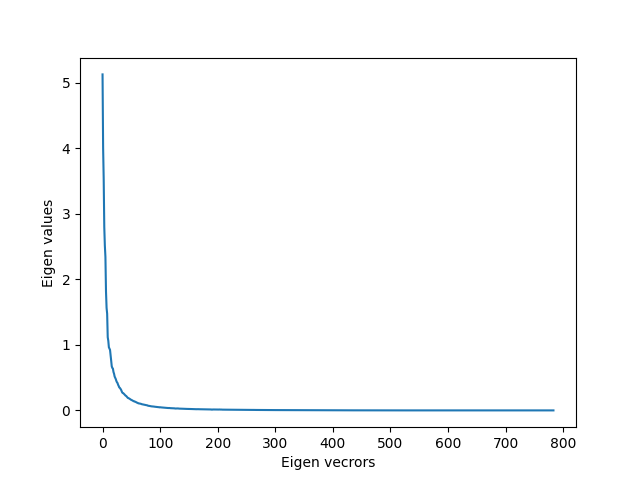
\includegraphics[width=3.6in]{eigen_values.png}	
	\caption{Eigen values of the correlation matrix $A$}
	\label{fig:eig_vals}
\end{figure}

\begin{figure}[!t]
	\centering
	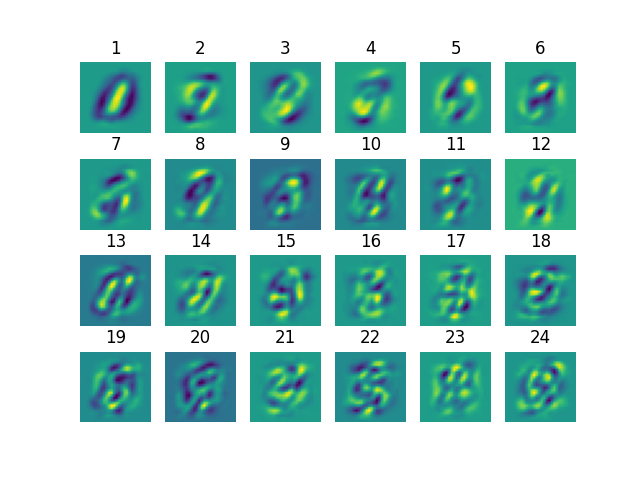
\includegraphics[width=3.6in]{eigen_vectors.png}
	
	\caption{Visualization of the eigen vectors of the principal components in descending order of eigenvalues}
	\label{fig:eig_vecs}
\end{figure}


\subsection{PCA vectors}

The plot of accuracy and computation time with different PCA vectors is presented in Fig. \ref{fig:pca_test}.
In the experiment, we used $K=5$, and 1000 training samples.
The accuracy is maximized at $M=50$, but the computation for inferring monotonously increases as PCA size increases.

\begin{figure}[!t]
	\centering
	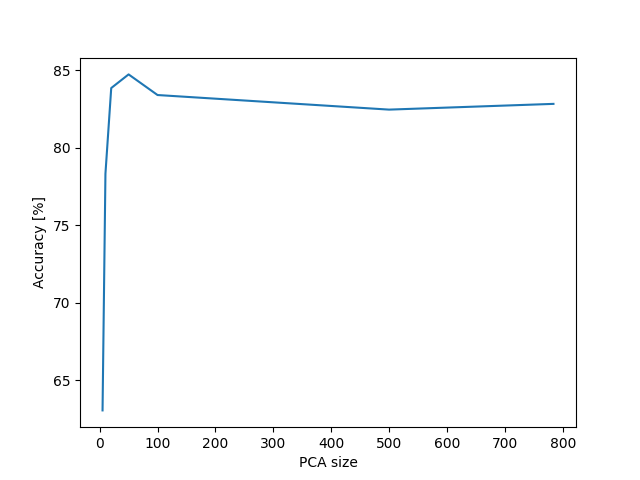
\includegraphics[width=3.6in]{pca_test.png}	
	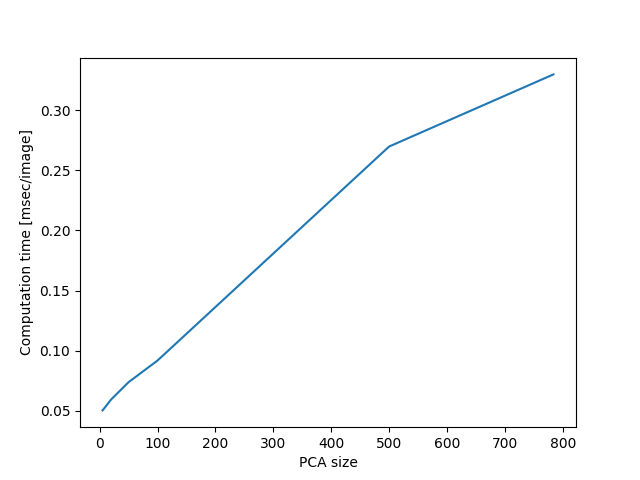
\includegraphics[width=3.6in]{pca_time.png}	
	\caption{Accuracy and computation time changes on PCA sizes: PCA sizes are chosen in [5, 10, 20, 50, 100, 500, 784].}
	\label{fig:pca_test}
\end{figure}


The reconstruction process stated above is tested with multiple sizes of PCA. 
For testing, we used the first 15 digit images from the test set.
The images of the reconstructed digits are presented at Fig. \ref{fig:pca_5} - \ref{fig:pca_784}. Note that when PCA size is 784, there no dimension is reduced when mapping, so it is equivalent to the original digit images.

\begin{figure}[!t]
	\centering
	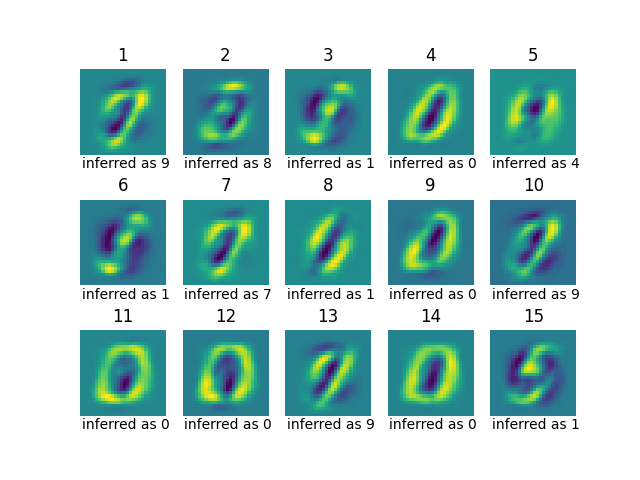
\includegraphics[width=3.6in]{reconst-PCA-5.png}	
	\caption{PCA size $M=5$}
	\label{fig:pca_5}
	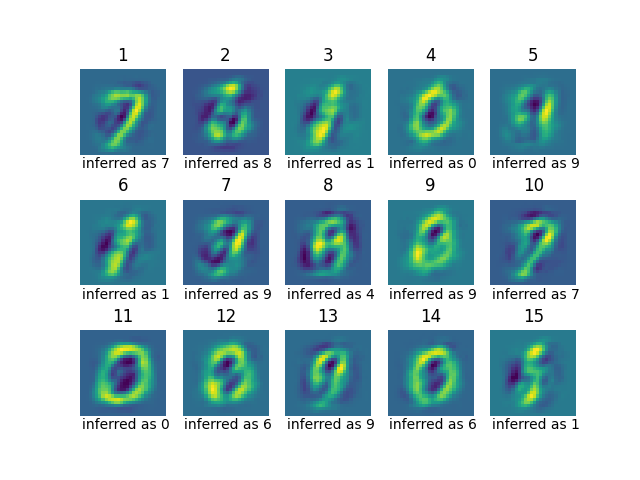
\includegraphics[width=3.6in]{reconst-PCA-10.png}
	\caption{PCA size $M=10$}
	\label{fig:pca_10}
	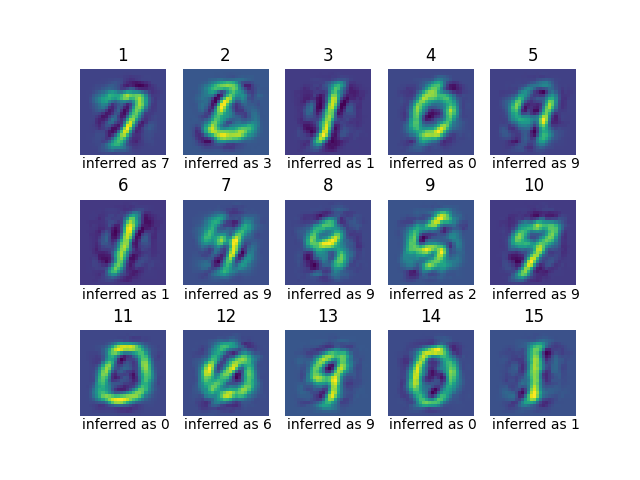
\includegraphics[width=3.6in]{reconst-PCA-20.png}
	\caption{PCA size $M=20$}
	\label{fig:pca_20}
\end{figure}


\begin{figure}[!t]
	\centering
	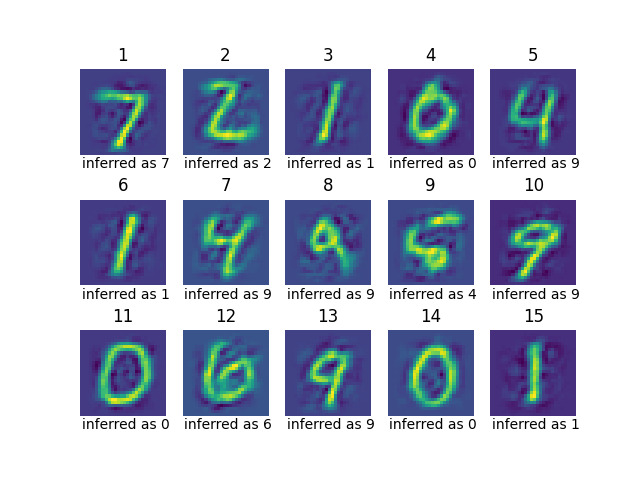
\includegraphics[width=3.6in]{reconst-PCA-50.png}
	\caption{PCA size $M=50$}
	\label{fig:pca_50}

	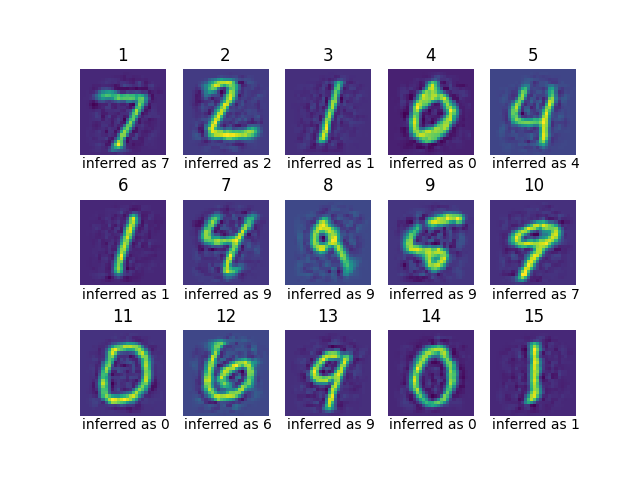
\includegraphics[width=3.6in]{reconst-PCA-100.png}	
	\caption{PCA size $M=100$}
	\label{fig:pca_100}

	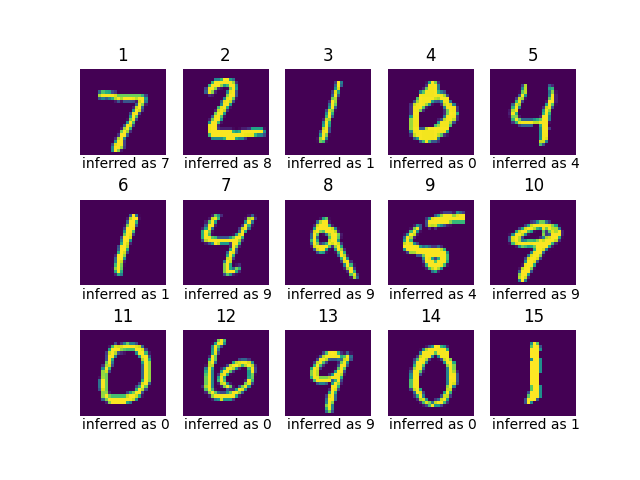
\includegraphics[width=3.6in]{reconst-PCA-784.png}
	\caption{PCA size $M=784$}
	\label{fig:pca_784}
\end{figure}


\subsection{K-Nearest Neighbors}

The plot of the accuracy of with different KNNs is presented in Fig. \ref{fig:knn_test}.
In the experiment, we used $M=24$, and 1000 training samples.
The accuracy for inferring worsens as KNN size increases, the computation time does not change much.

\begin{figure}[!t]
	\centering
	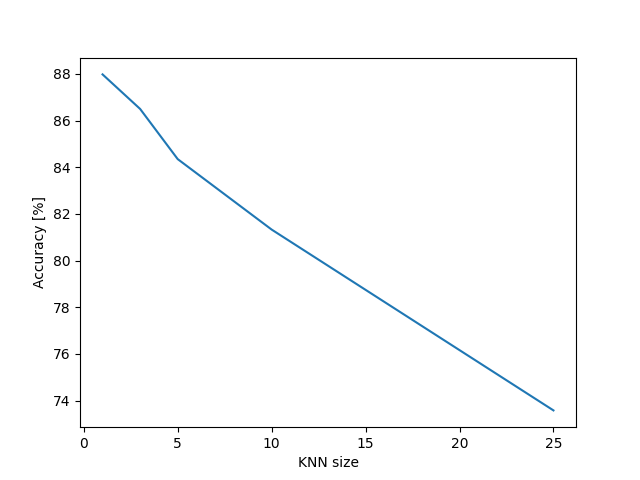
\includegraphics[width=3.6in]{knn_test.png}	
	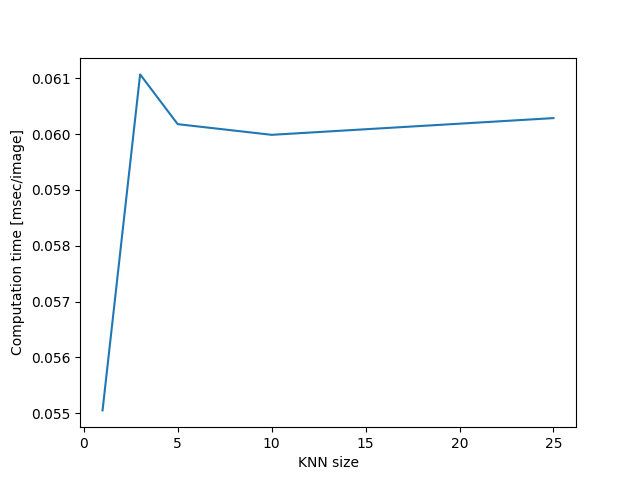
\includegraphics[width=3.6in]{knn_time.png}	
	\caption{Accuracy and computation time changes on KNN sizes: KNN sizes are chosen in [1, 3, 5, 10, 25].}
	\label{fig:knn_test}
\end{figure}


\subsection{Training samples}

The plot of accuracy of with different number of trainign samples is presented in Fig. \ref{fig:sample_test}.
In the experiment, we used $M=24$, and $K=5$.
There is trade-off in using a larger training sample size: the accuracy increases as a training sample size increases but computation time also increases linearly.

\begin{figure}[!t]
	\centering
	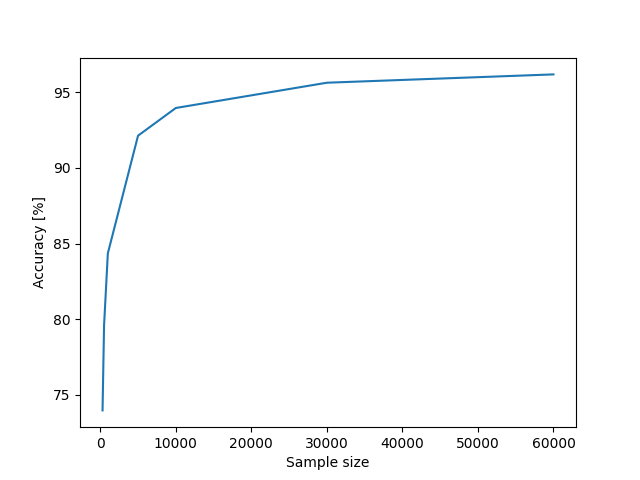
\includegraphics[width=3.6in]{sample_test.png}	
	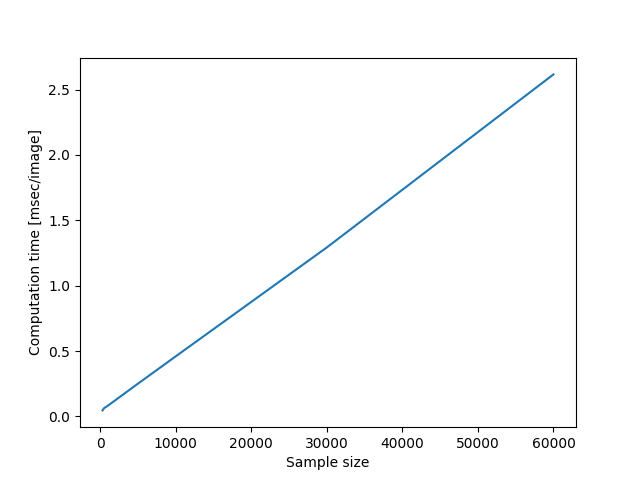
\includegraphics[width=3.6in]{sample_time.png}	
	\caption{Accuracy and computation time changes on training sample size: training sample sizes are chosen in [300, 500, 1000, 5000, 10000, 30000, 60000].}
	\label{fig:sample_test}
\end{figure}


\section{Summary} %Intermediate/Preliminary Results: State and evaluate your results upeto the milestone
The classifier method of PCA and KNN for classifying digit character images are implemented in the assignment. For evaluation, we used the MNIST dataset. From the results of the experiments, a smaller KNN size benefits the accuracy. However, for the PCA size, the accuracy peaked at $M=50$, This implies that enough number of feature is required for estimation but too many features distract the proper labels, which worsen the accuracy. On the other hand, a larger training size yields higher accuracy but also requires higher computation power.



%\section*{Acknowledgments}

%% Use plainnat to work nicely with natbib. 

\bibliographystyle{plainnat}
\bibliography{references}

\end{document}


